%% This LaTeX file is used to create graphs for the FinegrainedExperiments. It creates both a single pdf with all the graphs, and individual pdfs for each of the different graphs in the /finegrain_figures folder. If using pdflatex, this must be compiled using the --shell-escape option (for tikzexternalize to work).

\documentclass{article}

\usepackage{tikz}
\usepackage{pgfplots}

\usepgfplotslibrary{external}
\tikzexternalize

\begin{document}

%% The folder to use for the individual graphs
\tikzsetexternalprefix{finegrain_figures/}

\pgfplotsset{
  %% Macro to group results by qid
  discard if not/.style 2 args={
    x filter/.code={
      \edef\tempa{\thisrow{#1}}
      \edef\tempb{#2}
      \ifx\tempa\tempb
      \else
      \def\pgfmathresult{inf}
      \fi
    }
  },
  every axis/.append style={
    font=\large,
    line width=1pt,
    tick style={line width=0.8pt}
  }
}

%% Mark and line combinations to use
\pgfplotscreateplotcyclelist{originallinestyles}{
  {yellow,mark=square*},
  {orange,mark=diamond*},
  {brown,mark=triangle*},
  {red,mark=*},
  {olive,mark=pentagon*},
  {violet,mark=oplus*},
  {purple,mark=star},
  {blue,mark=x},
  {darkgray,mark=otimes*},
  {cyan,mark=+},
  {lime,mark=Mercedes star},
  {magenta,mark=asterisk}
}

%% Query numbers to plot
\newcommand{\ordersqueries}{4,13,21,7,10,5,3,12,18}
\newcommand{\customersqueries}{10,13,18}

%% Number of Unifications vs. Number of Constraints
\tikzsetnextfilename{Unif_vs_Const}
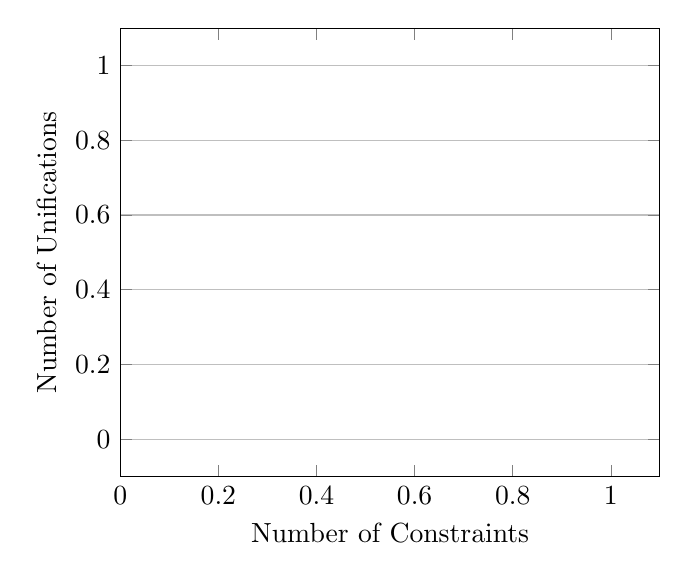
\begin{tikzpicture}
  \begin{axis} [
      xmin=0,
      xlabel=Number of Constraints,
      ylabel=Number of Unifications,
      ymajorgrids=true,
      legend style={
        legend pos=outer north east,
      },
      legend columns=12,
      transpose legend,
      cycle multi list={
        solid,{dashed,mark options={solid}}\nextlist
        originallinestyles
      },
      ]

    % Customer join results
    \foreach\g in \customersqueries{
      \addplot table [
        %% Only use lines for the current query
        discard if not={Qid}{\g},
        x=constraints,
        y=Runifications,
        col sep=comma
        ]
      {../../experiments/finegrain/customers-join.csv};
      \addlegendentryexpanded{CJ Q\g}
    }
    
    % Order join results
    \foreach\g in \ordersqueries{
      \addplot table [
        discard if not={Qid}{\g},
        x=constraints,
        y=Runifications,
        col sep=comma
        ]
        {../../experiments/finegrain/orders-join.csv};
      \addlegendentryexpanded{OJ Q\g}
    }

    % Customer no join results
    \foreach\g in \customersqueries{
      \addplot table [
        discard if not={Qid}{\g},
        x=constraints,
        y=Runifications,
        col sep=comma
        ]
      {../../experiments/finegrain/customers-nojoin.csv};
      \addlegendentryexpanded{CW Q\g}
    }

    % Order no join results
    \foreach\g in \ordersqueries{
      \addplot table [
        discard if not={Qid}{\g},
        x=constraints,
        y=Runifications,
        col sep=comma
        ]
      {../../experiments/finegrain/orders-nojoin.csv};
      \addlegendentryexpanded{OW Q\g}
    }

  %% Clear legend
  \legend{}
    
  \end{axis}
\end{tikzpicture}

%% Slowdown Multiplier vs. Number of Constraints
\tikzsetnextfilename{Slowdown_vs_Const}
\begin{tikzpicture}
  \begin{axis} [
      xmin=0,
      xtick distance=100,
      ytick distance=2,
      xlabel=Number of Constraints,
      ylabel=Slowdown Multiplier,
      ymajorgrids=true,
      legend style={
        legend pos=outer north east,
      },
      legend columns=12,
      transpose legend,
      cycle multi list={
        solid,{dashed,mark options={solid}}\nextlist
        originallinestyles
      },
      ]

    % Customer join results
    \foreach\g in \customersqueries{
      \addplot table [
        discard if not={Qid}{\g},
        x=constraints,
        y expr=\thisrow{Rexecution} / \thisrow{Qexecution},
        col sep=comma
        ]
      {../../experiments/finegrain/customers-join.csv};
      \addlegendentryexpanded{CJ Q\g}
    }
    
    % Order join results
    \foreach\g in \ordersqueries{
      \addplot table [
        discard if not={Qid}{\g},
        x=constraints,
        y expr=\thisrow{Rexecution} / \thisrow{Qexecution},
        col sep=comma
        ]
        {../../experiments/finegrain/orders-join.csv};
      \addlegendentryexpanded{OJ Q\g}
    }

    % Customer no join results
    \foreach\g in \customersqueries{
      \addplot table [
        discard if not={Qid}{\g},
        x=constraints,
        y expr=\thisrow{Rexecution} / \thisrow{Qexecution},
        col sep=comma
        ]
      {../../experiments/finegrain/customers-nojoin.csv};
      \addlegendentryexpanded{CW Q\g}
    }

    % Order no join results
    \foreach\g in \ordersqueries{
      \addplot table [
        discard if not={Qid}{\g},
        x=constraints,
        y expr=\thisrow{Rexecution} / \thisrow{Qexecution},
        col sep=comma
        ]
      {../../experiments/finegrain/orders-nojoin.csv};
      \addlegendentryexpanded{OW Q\g}
    }

  %% Clear legend
  \legend{}
    
  \end{axis}
\end{tikzpicture}


%% Slowdown Multiplier vs. Number of Unifications
\tikzsetnextfilename{Slowdown_vs_Unif}
\begin{tikzpicture}
  \begin{axis} [
      xmin=0,
      ytick distance=2,
      xlabel=Number of Unifications,
      ylabel=Slowdown Multiplier,
      ymajorgrids=true,
      legend style={
        legend pos=outer north east,
      },
      legend columns=12,
      transpose legend,
      cycle multi list={
        solid,{dashed,mark options={solid}}\nextlist
        originallinestyles
      },
      ]

    % Customer join results
    \foreach\g in \customersqueries{
      \addplot table [
        discard if not={Qid}{\g},
        x=Runifications,
        y expr=\thisrow{Rexecution} / \thisrow{Qexecution},
        col sep=comma
        ]
      {../../experiments/finegrain/customers-join.csv};
      \addlegendentryexpanded{CJ Q\g}
    }
    
    % Order join results
    \foreach\g in \ordersqueries{
      \addplot table [
        discard if not={Qid}{\g},
        x=Runifications,
        y expr=\thisrow{Rexecution} / \thisrow{Qexecution},
        col sep=comma
        ]
        {../../experiments/finegrain/orders-join.csv};
      \addlegendentryexpanded{OJ Q\g}
    }

    % Customer no join results
    \foreach\g in \customersqueries{
      \addplot table [
        discard if not={Qid}{\g},
        x=Runifications,
        y expr=\thisrow{Rexecution} / \thisrow{Qexecution},
        col sep=comma
        ]
      {../../experiments/finegrain/customers-nojoin.csv};
      \addlegendentryexpanded{CW Q\g}
    }

    % Order no join results
    \foreach\g in \ordersqueries{
      \addplot table [
        discard if not={Qid}{\g},
        x=Runifications,
        y expr=\thisrow{Rexecution} / \thisrow{Qexecution},
        col sep=comma
        ]
      {../../experiments/finegrain/orders-nojoin.csv};
      \addlegendentryexpanded{OW Q\g}
    }

  %% Clear legend
  \legend{}
  
  \end{axis}
\end{tikzpicture}


%% Rewriting time vs. Number of Constraints
\tikzsetnextfilename{Rewriting_vs_Const}
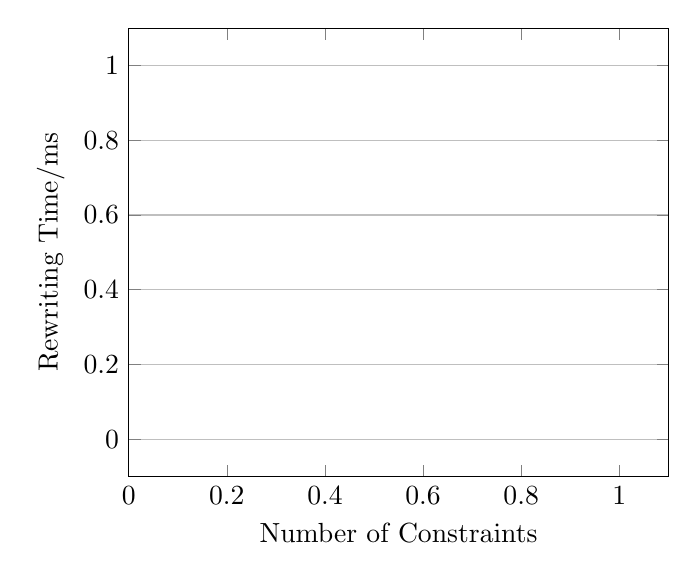
\begin{tikzpicture}
  \begin{axis} [
      xmin=0,
      xlabel=Number of Constraints,
      ylabel=Rewriting Time/ms,
      ymajorgrids=true,
      legend style={
        legend pos=outer north east,
      },
      legend columns=12,
      transpose legend,
      cycle multi list={
        solid,{dashed,mark options={solid}}\nextlist
        originallinestyles
      },
      ]

    % Customer join results
    \foreach\g in \customersqueries{
      \addplot table [
        discard if not={Qid}{\g},
        x=numberconstraints,
        y expr=\thisrow{rewritingtimenano} / 1000000,
        col sep=comma
        ]
      {../../experiments/finegrain/customers-rewritings-join.csv};
      \addlegendentryexpanded{CJ Q\g}
    }
    
    % Order join results
    \foreach\g in \ordersqueries{
      \addplot table [
        discard if not={Qid}{\g},
        x=numberconstraints,
        y expr=\thisrow{rewritingtimenano} / 1000000,
        col sep=comma
        ]
        {../../experiments/finegrain/order-rewritings-join.csv};
      \addlegendentryexpanded{OJ Q\g}
    }

    % Customer no join results
    \foreach\g in \customersqueries{
      \addplot table [
        discard if not={Qid}{\g},
        x=numberconstraints,
        y expr=\thisrow{rewritingtimenano} / 1000000,
        col sep=comma
        ]
      {../../experiments/finegrain/customers-rewritings-nojoin.csv};
      \addlegendentryexpanded{CW Q\g}
    }

    % Order no join results
    \foreach\g in \ordersqueries{
      \addplot table [
        discard if not={Qid}{\g},
        x=numberconstraints,
        y expr=\thisrow{rewritingtimenano} / 1000000,
        col sep=comma
        ]
      {../../experiments/finegrain/order-rewritings-nojoin.csv};
      \addlegendentryexpanded{OW Q\g}
    }
    
  \end{axis}
\end{tikzpicture}

\end{document}

%%% Local Variables:
%%% mode: latex
%%% TeX-master: t
%%% TeX-command-extra-options: "-shell-escape"
%%% End:
